% Author: Joshua Payne
%\documentclass{article}
\documentclass[class=minimal,border=0pt]{standalone}
%\usepackage{beamerposter}
%\setlength{\paperwidth}{29.7cm}
%\setlength{\paperheight}{21.0cm}
%\setlength{\textwidth}{28.7cm}
%\setlength{\textheight}{20.0cm} 

\usepackage[usenames,dvipsnames]{xcolor}
\usepackage{tikz}


\usepackage{ifthen}
\usetikzlibrary{chains,fit,shapes}

\begin{document}



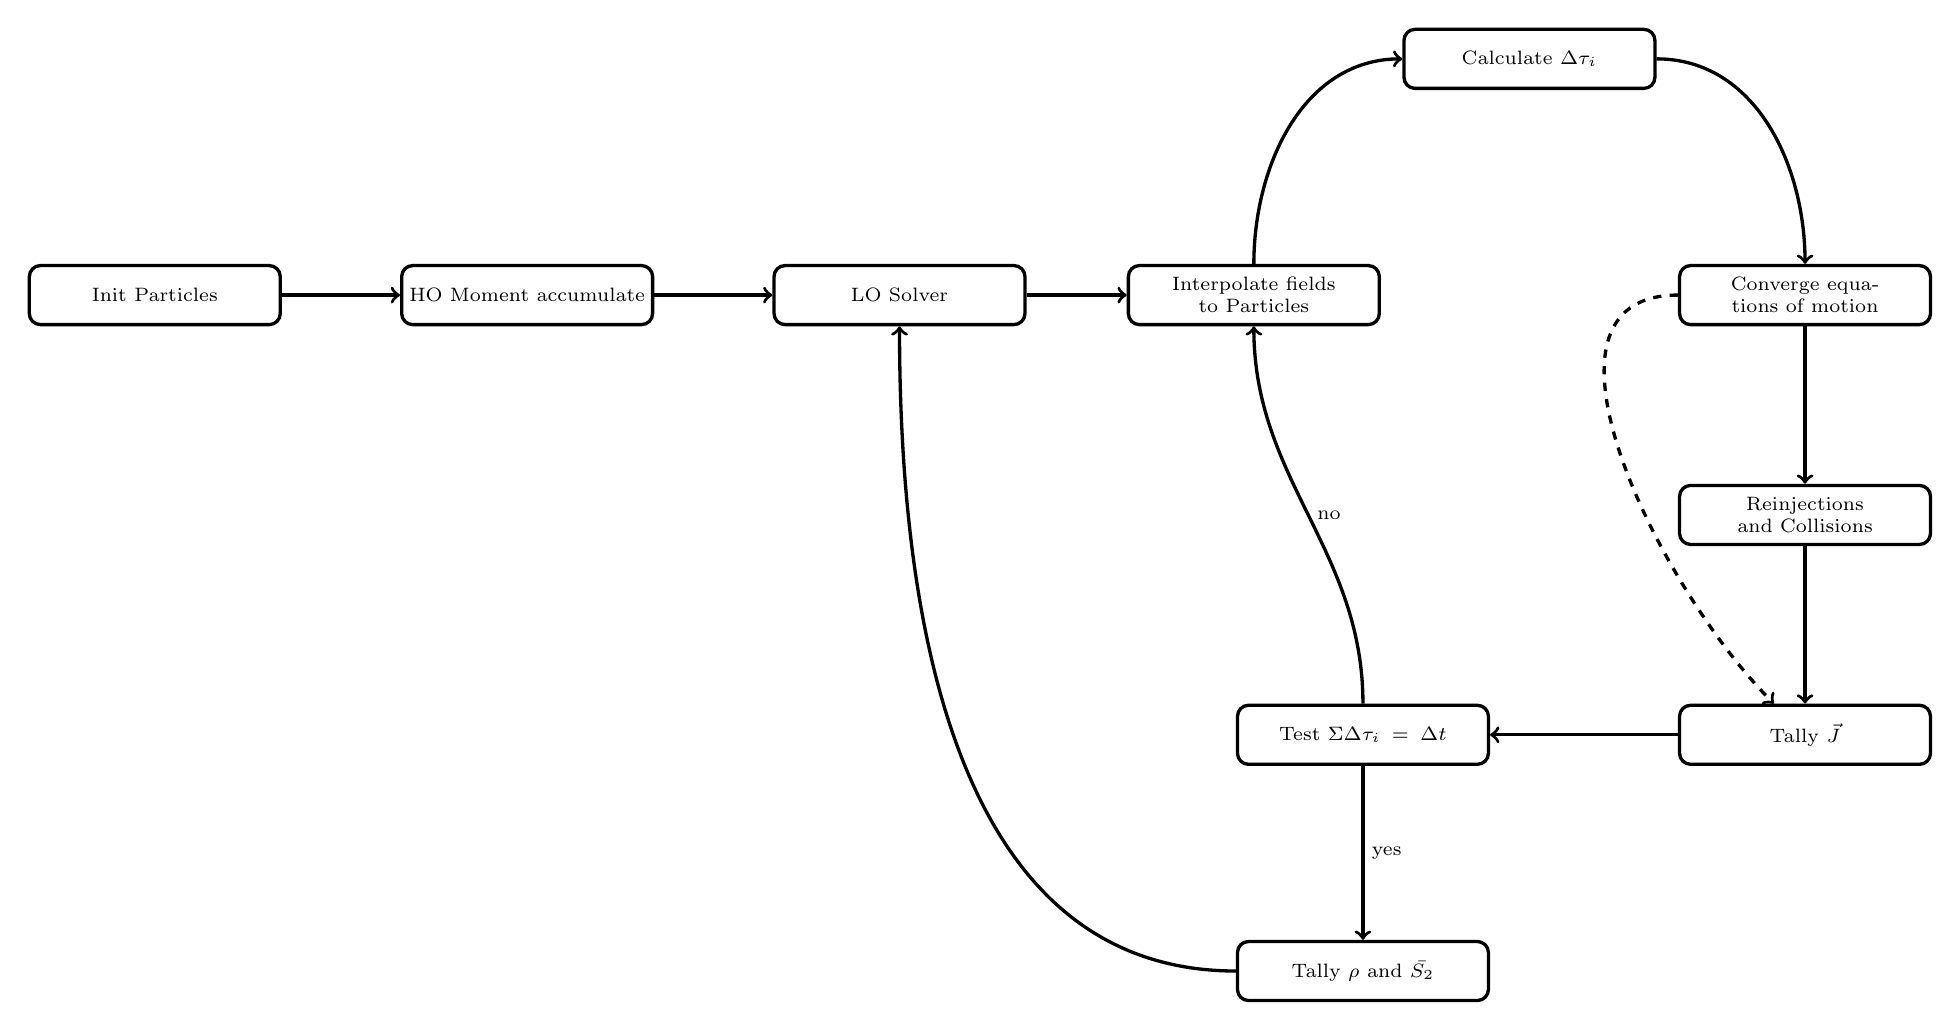
\begin{tikzpicture}[remember picture=false]
		\tikzstyle{every path}=[very thick]
		\tikzstyle{MainSty}=[->,dashdotted]
		\tikzstyle{CollSty}=[->,color=Emerald,densely dashdotted]
		\tikzstyle{ReinSty}=[->,color=Maroon,dashed]

		\edef\sizetape{3.0cm}
		\tikzstyle{tmtape}=[draw,
								  minimum width=\sizetape,
								  minimum height=0.75cm,
								  text width=3.0cm,
								  rounded corners,
								  align=center]
		\tikzstyle{tmtape1}=[draw,
									minimum height=\sizetape,
									minimum width=0.5cm,
									textwidth=0.5cm]
		\tikzstyle{tmhead}=[arrow box,draw,minimum size=3.0cm,arrow box
		arrows={east:.25cm}]

		\tikzstyle{cfill0}=[color=Purple]
		\tikzstyle{cfill1}=[color=SkyBlue]
		\tikzstyle{cfill2}=[color=Maroon]
		\tikzstyle{cfill3}=[color=Emerald]


\def\MainArray{1,...,10}
\def\DeadArray{2,4,8}
\def\SplitArray{{1,3,3,6,5,6,7,9,9,10}}

\scriptsize

\newcounter{prim@a}
\newcounter{prim@b}
\newcounter{prim@c}
\newcounter{prim@d}
\newcommand*{\pshiftmm}{(-2.0mm,-2.0mm)}
\newcommand*{\pshiftpm}{(2.0mm,-2.0mm)}
\newcommand*{\pshiftmp}{(-2.0mm,2.0mm)}
\newcommand*{\pshiftpp}{(2.0mm,2.0mm)}

% MPI Level
\begin{scope}[xshift=-2.0cm,start chain=1,node distance=1.5cm]

	\node [on chain=1,tmtape] (init) {Init Particles};
	\node [on chain=1,tmtape] (init2) {HO Moment accumulate};
	\node [on chain=1,tmtape] (LO) {LO Solver};

\end{scope}


\begin{scope}[xshift=2.0cm,start chain=1 going below,start chain=2 going left,node distance=2cm]

	\node [tmtape,xshift=4.5cm] at (LO) (intrpfields) {Interpolate fields to Particles};
	\node [tmtape,shift={(3.5cm,3.0cm)}] at (intrpfields) (time) {Calculate $\Delta\tau_i$};
	\node [on chain=1,tmtape,shift={(7.0cm,0.0cm)}] at (intrpfields) (push) {Converge equations of motion};
	\node [on chain=1,tmtape] (reinj) {Reinjections and Collisions};
	\node [on chain=1,on chain=2,tmtape] (tallies) {Tally $\vec{J}$ };
	\node [on chain=2,tmtape,xshift=-2.0cm] at (tallies) (subexit) {Test $\Sigma\Delta\tau_i = \Delta t$};
	\node [tmtape,yshift=-3cm] at (subexit) (ctally) {Tally $\rho$ and $\bar{S_2}$};
	
	
\end{scope}

	\path[->] (init) edge (init2);
	\path[->] (init2) edge (LO);
	\path[->] (LO) edge (intrpfields);
	\path[->] (intrpfields) edge[out=90,in=180] (time);
	\path[->] (time) edge[out=0,in=90] (push);
	\path[->] (push) edge[out=-90,in=90] (reinj);
	\path[->] (reinj) edge[out=-90,in=90] (tallies);
	\path[->] (tallies) edge (subexit);
	\path[->] (subexit) edge[out=90,in=-90] node[right] {no} (intrpfields);
	\path[->] (subexit) edge node[right] {yes} (ctally);
	\path[->] (ctally) edge[out=180,in=-90] (LO);
	\path[->] (push) edge[out=180,dashed] (tallies);



\end{tikzpicture}
\end{document}

